\documentclass[10pt]{IEEEtran}
% \usepackage{IEEEtran}
\usepackage{amsmath,amsfonts}
\usepackage{etoolbox}
\usepackage{array}
\usepackage{pifont}
\usepackage[caption=false,font=normalsize,labelfont=sf,textfont=sf]{subfig}
\usepackage{textcomp}
\usepackage{stfloats}
\usepackage{url}
\usepackage{verbatim}
\usepackage{graphicx}
\usepackage{cite}
\usepackage{float}
\usepackage{adjustbox}
\usepackage{caption}
\captionsetup[table]{labelformat=simple, labelsep=newline,justification=centering}

\usepackage[pagebackref,breaklinks,colorlinks,colorlinks=true]{hyperref}
\usepackage[capitalize]{cleveref}

\usepackage{booktabs,makecell, multirow, tabularx, tabularray}
\usepackage{latexsym}
\usepackage{algorithmic,algorithm}
\usepackage{subcaption}
\usepackage{graphbox}
\usepackage{xspace} 

\usepackage{lipsum}

\makeatletter
\DeclareRobustCommand\onedot{\futurelet\@let@token\@onedot}
\def\@onedot{\ifx\@let@token.\else.\null\fi\xspace}
\def\eg{\emph{e.g}\onedot} \def\Eg{\emph{E.g}\onedot}
\def\ie{\emph{i.e}\onedot} \def\Ie{\emph{I.e}\onedot}
\def\cf{\emph{cf}\onedot} \def\Cf{\emph{Cf}\onedot}
\def\etc{\emph{etc}\onedot} \def\vs{\emph{vs}\onedot}
\def\wrt{w.r.t\onedot} \def\dof{d.o.f\onedot}
\def\iid{i.i.d\onedot} \def\wolog{w.l.o.g\onedot}
\def\etal{\emph{et al}\onedot}
\def\figureautorefname{Fig.}
\def\figureautorefnames{Figs.}
\crefformat{figure}{#2\figureautorefname~#1#3}
\def\tableautorefname{Tab.}
\crefformat{table}{#2\tableautorefname~#1#3}
\renewcommand{\thetable}{\arabic{table}}
% \setcounter{table}{1}
\makeatother
% \usepackage{bibdata, citation, bibstyle}
\hyphenation{op-tical net-works semi-conduc-tor IEEE-Xplore}
% updated with editorial comments 8/9/2021
\DeclareRobustCommand*{\IEEEauthorrefmark}[1]{%
    \raisebox{0pt}[0pt][0pt]{\textsuperscript{\footnotesize\ensuremath{#1}}}}
\captionsetup[figure]{name={Fig.},labelsep=period}


% \captionsetup[table]{labelfont={f},name={Tab.},labelsep=period}
\begin{document}

\title{I Love Music}


\author{
        John Mayer\thanks{* BB King, is the corresponding author.}\thanks{John Mayer is with School of XXX, University of XXX, XXXX 100049, USA, 
        and also with XXXX, XXX, XXX 100101, USA (e-mail: likai211@mails.ucas.ac.cn)}, 
        B.B. King\textsuperscript{*},
        and Eric Clapton
} 


% The paper headers
\markboth{Journal of \LaTeX\ Template,~Vol.~14, No.~16, October~2023}%
{Shell \MakeLowercase{\textit{et al.}}: A Sample Article Using IEEEtran.cls for IEEE Journals}

% \IEEEpubid{0000--0000/00\$00.00~\copyright~2021 IEEE}
% Remember, if you use this you must call \IEEEpubidadjcol in the second
% column for its text to clear the IEEEpubid mark.

\maketitle
\begin{abstract}
\lipsum[1]
\end{abstract}

\begin{IEEEkeywords}
    Guitar, Band, Music
\end{IEEEkeywords}
    
% \IEEEpubidadjcol
% \section{Introduction}
\section{Introduction}
\label{sec:Intro}
\limsum[3-5]
\begin{figure*}[htbp]
	\centering
	\begin{minipage}{0.24\linewidth}
		\vspace{4pt}
		\centerline{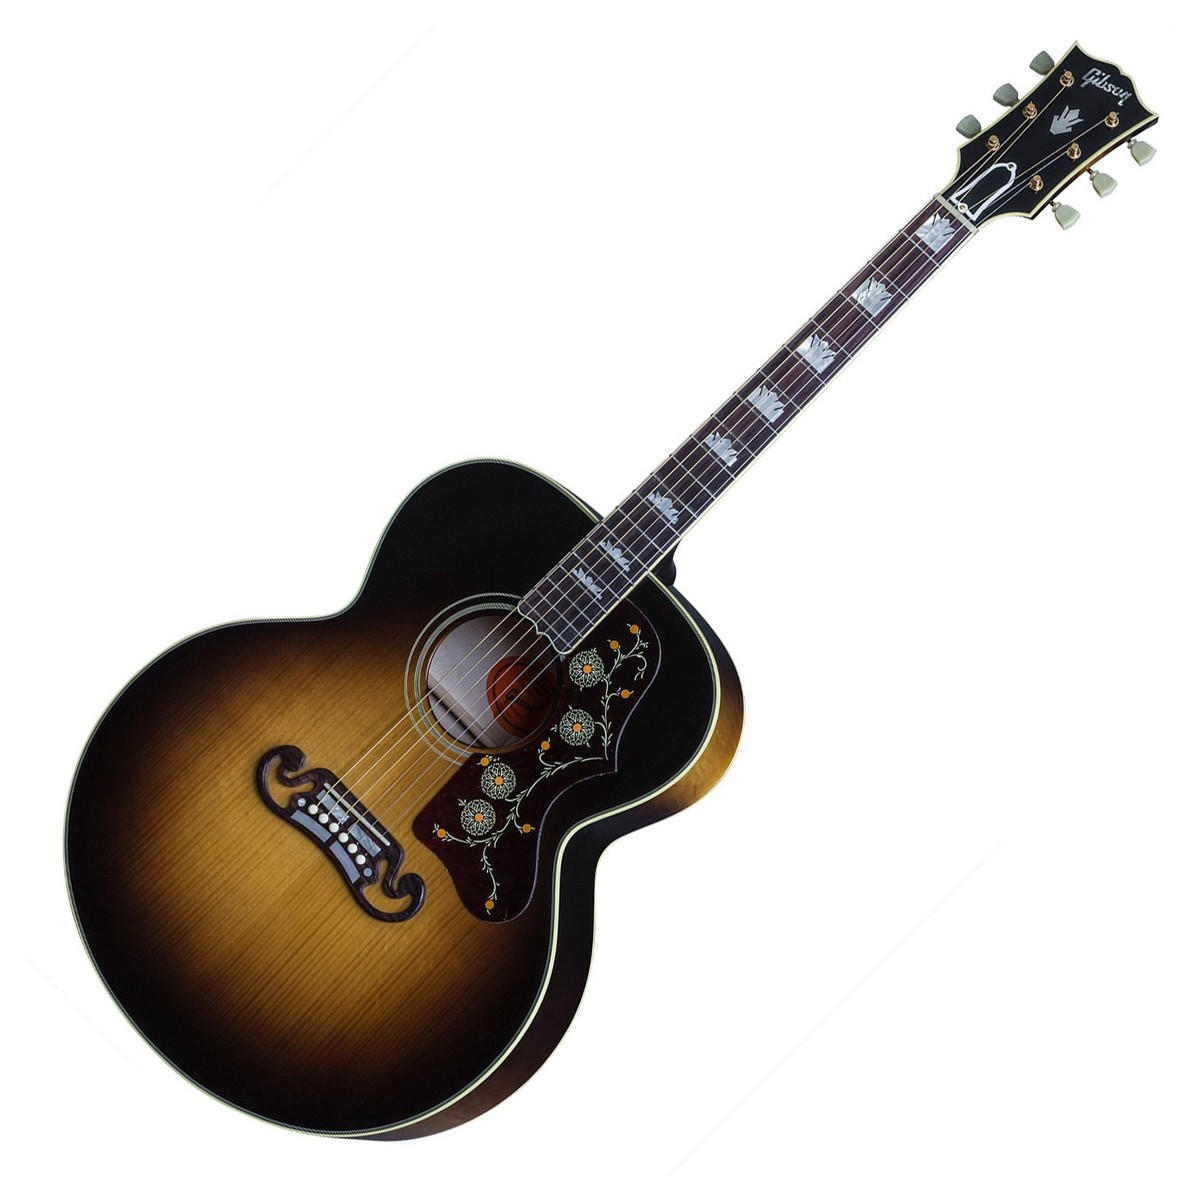
\includegraphics[width=\textwidth]{intro/Gibson.jpg}}
        \centerline{Gibson} 
	\end{minipage}
	\begin{minipage}{0.24\linewidth}
		\vspace{4pt}
		\centerline{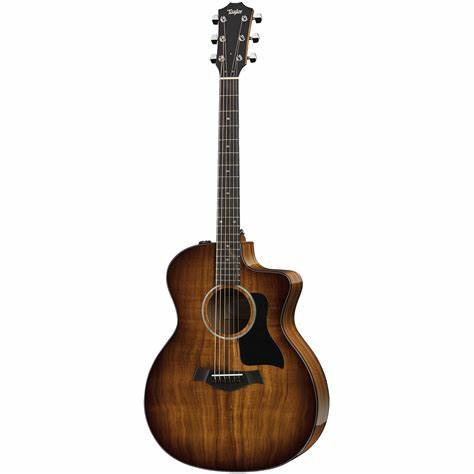
\includegraphics[width=\textwidth]{intro/Tylor.jpg}}
		\centerline{Tylor}
	\end{minipage}
	\begin{minipage}{0.24\linewidth}
		\vspace{4pt}
		\centerline{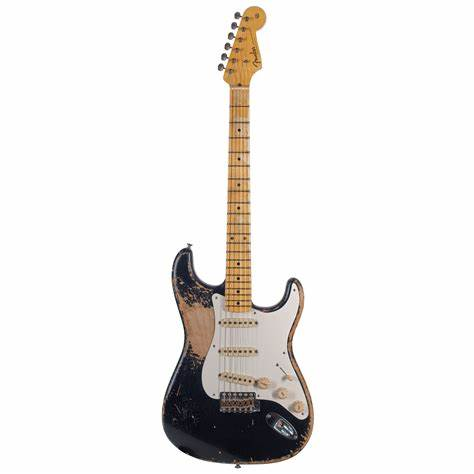
\includegraphics[width=\textwidth]{intro/Fender.jpg}}
		\centerline{Fender}
	\end{minipage}
    \begin{minipage}{0.24\linewidth}
		\vspace{4pt}
		\centerline{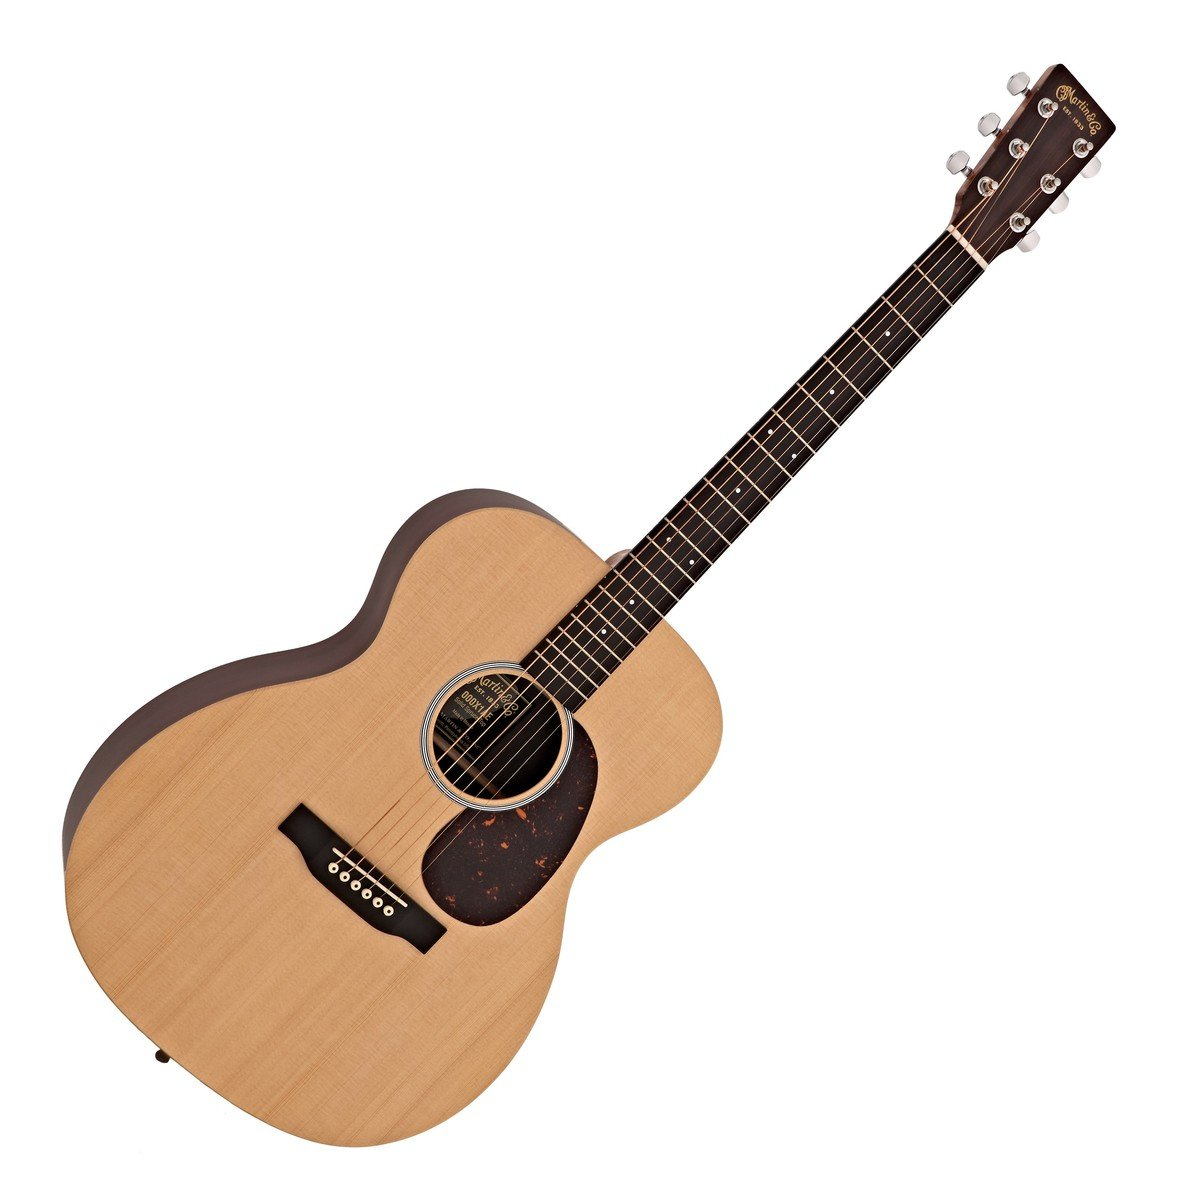
\includegraphics[width=\textwidth]{intro/Martin.jpg}}
		\centerline{Martin}
	\end{minipage}
	\caption{World famous guitar brands.}
	\label{fig.0}
\end{figure*}

\lipsum[7-8]


In summary, our contribution is as follows:
\begin{enumerate}
 \item[$\bullet$] JM is cool. 
 \item[$\bullet$] BB King is cool. 
 \item[$\bullet$] EC is cool. 
\end{enumerate}
%-------------------------------------------------------------------------
% \appendix
% \clearpage
% % \setcounter{page}{1}
% \maketitlesupplementary


\section{Related Work}
\label{sec:RW}
\lipsum[3-5]

{\bf WDa WARE :} 
\lipsum[3-5]

{\bf WDa WARE :} 
\lipsum[3-5]

{\bf WDa WARE :} 
\lipsum[3-5]
\section{Methodology}
\cref{subsec:1} introduces XX.
\cref{subsec:2} describes XX.
\cref{subsec:3} introduces XX.
\cref{subsec:4} describes XX.
\cref{subsec:5} describes XX.
%-------------------------------------------------------------------------
\subsection{Problem formulation}
\label{subsec:1}
\lipsum[1]
\begin{equation}
  \begin{cases}
  D = \{(I_i, P_i, T_i); i=1,2,\ldots,N\} \\
  P_i \in \{\text{A,B,C}\} \\
  T_i = MODEL(I_i, P_i), \quad i=1,2,\ldots,N \\
  \end{cases}
  \label{eq:1}
\end{equation}
\lipsum[4]
%-------------------------------------------------------------------------
\subsection{wdada wad fawefa}
\label{subsec:2}
\lipsum[4]

%-------------------------------------------------------------------------
\subsubsection{Podaiojndoa awed jmp}
\lipsum[4]
{\bf Wda wdgr gyuykjy:} \lipsum[1]

{\bf iojicbyu ujie:} \lipsum[1]
%-------------------------------------------------------------------------
\subsubsection{Oftwd r wfda }
\lipsum[4]

\begin{algorithm}[!hbp]
	\caption{daw da fghgrt s}
    \label{sdms}
    \begin{algorithmic}
      \REQUIRE dwa : $O:\{\theta_i, \rho_i, \vec p_i=(x_i, y_i) | i = 1,2,...,n\}$
        \STATE wad  $O$: $\mu \gets \frac{\sum_{i=1}^{n} \rho_i}{n}$ 
        \STATE wa  $O$: $\sigma^2 \gets \mu \frac{\sum_{i=1}^{n} (\rho_i - \mu)^2}{n-1}$  
        \STATE urtrhh:  $r = \mu+ \alpha \times \sigma$
        \STATE erwww: $\mathcal{D}:\{d_i = e^{-\frac{(\rho_i - r)^2}{2\sigma^2} }| i = 1,2,...,n\}$
        \STATE turtyhr: $x_s = \frac{\sum_{i=1}^{n} \omega_i x_i}{\sum_{i=1}^{n}\omega_i}$; $y_s = \frac{\sum_{i=1}^{n} \omega_i y_i}{\sum_{i=1}^{n}\omega_i}$
        \STATE 3wrwrf: $\vec p_u = (x_u, y_u)$, \\
              \hspace{2em}where: $x_u = \frac{x_s}{\sqrt{{x_s}^2 + {y_s}^2}}$; $y_u = \frac{y_s}{\sqrt{{x_s}^2 + {y_s}^2}}$
        \STATE w3rwrrwr: $\vec f_i = (1-d_i)\times \vec p_i + d_i \rho_i \times \vec p_u$
        \ENSURE 3rwrw: $O:\{\vec f_i | i = 1,2,...,n\}$
    \end{algorithmic}
\end{algorithm}
In \cref{sdms}, w3rwf. 
The \( \alpha \) waed okopfs. 
The \( \omega_i \) 3wrw3rw. 



\subsection{okpawdiodaw}
\label{subsec:4}
\lipsum[4]

\begin{figure}[H]
  \centering
  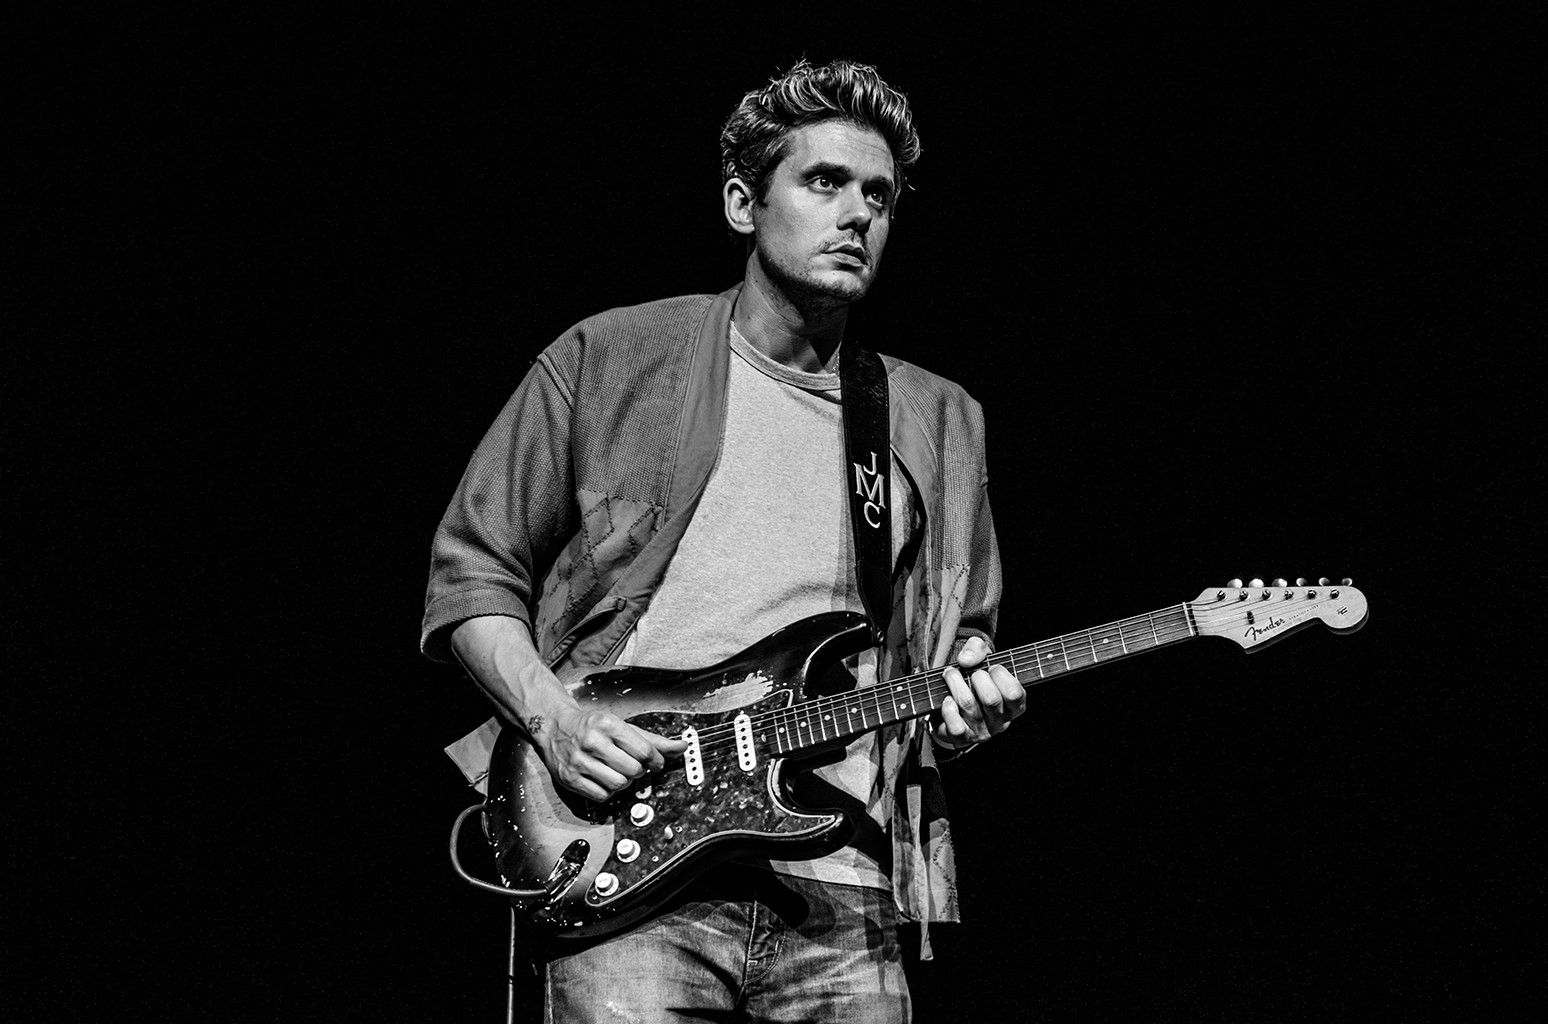
\includegraphics[width=\linewidth]{author/JM.jpg}
  \caption{COOOOOOOOOOOOOOOOOOOOOOL!!!!}
  \label{fig:3}
\end{figure}

\lipsum[4]

\subsection{Redow d asda}
\label{subsec:5}
\lipsum[4]
\cite[myjournal]{myjournal}
\lipsum[4]

\section{Experiment}
\lipsum[3-5]
\subsection{Main result}
\begin{table*}[htbp]
  % \begin{center}
    \centering
  \caption{\lipsum[1]\cite{a12}.}
  \label{tab.1}
  \resizebox{\linewidth}{!}{
  \begin{tabular}{cc|ccccccccccccc}
    \toprule
    {\textbf{Model}} & ~ & \textbf{0,10} & \textbf{10,20} & \textbf{20,30} & \textbf{30,40} & \textbf{40,50} & \textbf{50,60} & \textbf{60,70} & \textbf{70,80} & \textbf{80,90} & \textbf{90,100} & \textbf{100,\(\infty\) } & \textbf{$m$\(\mathcal{L}\)} & \textbf{$a$\(\mathcal{L}\)} \\ \hline
        ~& $A$ & 5.48 & 4.34 & 6.39 & 6.80 & 8.41 & 11.8 & 15.6 & 20.3 & 17.2 & \textbf{18.2} & \textbf{53.9} & 15.4 & 6.12 \\ 
        LOFT & $A$ & 4.15 & 2.75 & 4.51 & 5.18 & 6.52 & 8.70 & 12.2 & 16.7 & 12.9 & \textbf{14.4} & \textbf{49.9} & 12.6 & 4.51\\ 
        ~& $A$ & 0.55 & 0.21 & 0.17 & 0.11 & 0.10 & 0.14 & 0.15 & 0.16 & 0.13 & 0.13 & 0.15 & 0.18 & 0.32 \\ \hline
        \multirow{3}{*}{\thead{Cas.\\LOFT}}& $V$ & 5.62 & 4.12 & \textbf{5.42} & 6.11 & 7.90 & 12.8 & 17.3 & 22.7 & 17.9 & 18.7 & 55.3 & 15.8 & 5.97   \\ 
         &$A$ & 4.28 & 2.66 & \textbf{3.71} & 4.72 & 6.30 & 10.8 & 15.2 & 20.2 & 14.1 & 14.8 & 51.3 & 13.5 & 4.48 \\
         &$A$ & 0.55 & 0.19 & 0.15 & 0.09 & 0.09 & 0.14 & 0.13 & 0.13 & 0.14 & 0.15 & 0.14 & 0.17 & 0.31 \\ \hline
         ~& $A$ & \textbf{4.01} & \textbf{3.71} & 5.55 & \textbf{6.10} & \textbf{7.58} & \textbf{9.18} & \textbf{12.5} & \textbf{16.9} & \textbf{15.1} & 21.2 & 61.4 & \textbf{14.8} & \textbf{5.08} \\ 
        Ours& $A$ & \textbf{3.20} & \textbf{2.55} & 4.14 & \textbf{4.96} & \textbf{6.14} & \textbf{7.77} & \textbf{10.8} & \textbf{15.9} & \textbf{13.8} & 19.5 & 60.1 & \textbf{13.5} & \textbf{4.03} \\
        & $A$ & \textbf{0.37} & \textbf{0.15} & \textbf{0.14} & \textbf{0.08} & \textbf{0.08} & \textbf{0.07} & \textbf{0.08} & \textbf{0.06} & \textbf{0.06} & \textbf{0.10} & \textbf{0.11} & \textbf{0.12} & \textbf{0.22} \\ \bottomrule
    \end{tabular}
  }
  % \end{center}
\end{table*}
\cref{tab.1} \lipsum[4]

\section{Ablation}
\label{sec:ablation}
\lipsum[4]
\section{Discussion}
% In this paper, we propose a decoupling model, named OBM, for BFE problem. OBM is still powerful in our generalization test. DNMS algorithms,
% based on common patterns of predicting offset, work for all models. 

\subsection{Why does XXX?}
\label{whybetter1}
\lipsum[4]

\subsection{Why does XXX?}
\label{whybetter2}
\lipsum[4]

\subsection{Why does XXX?}
\label{whybetter3}
\lipsum[4]

\section{Conclusion}
limsum[3-5]
% \usepackage[backend=bibtex]{biblatex}
\bibliographystyle{IEEEtran}
\bibliography{main} 


\begin{IEEEbiography}[{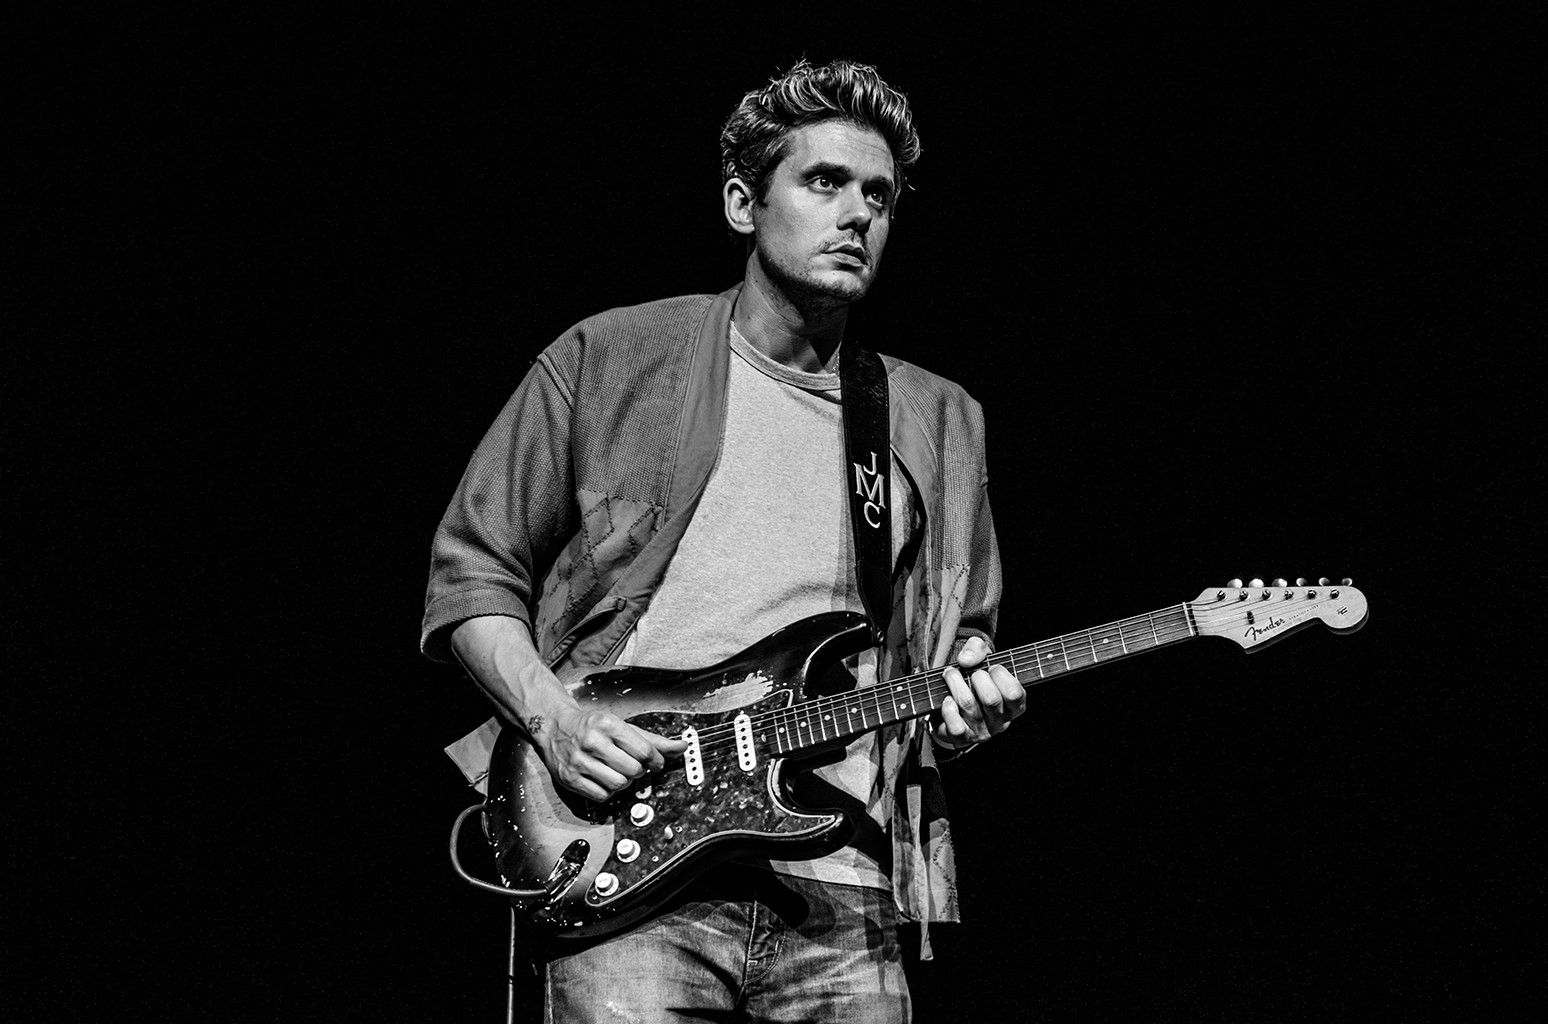
\includegraphics[width=1in,height=1.25in,clip,keepaspectratio]{author/JM.jpg}}]{John Mayer}\\
       is my guitar hero. I love his music.
\end{IEEEbiography}
\begin{IEEEbiography}[{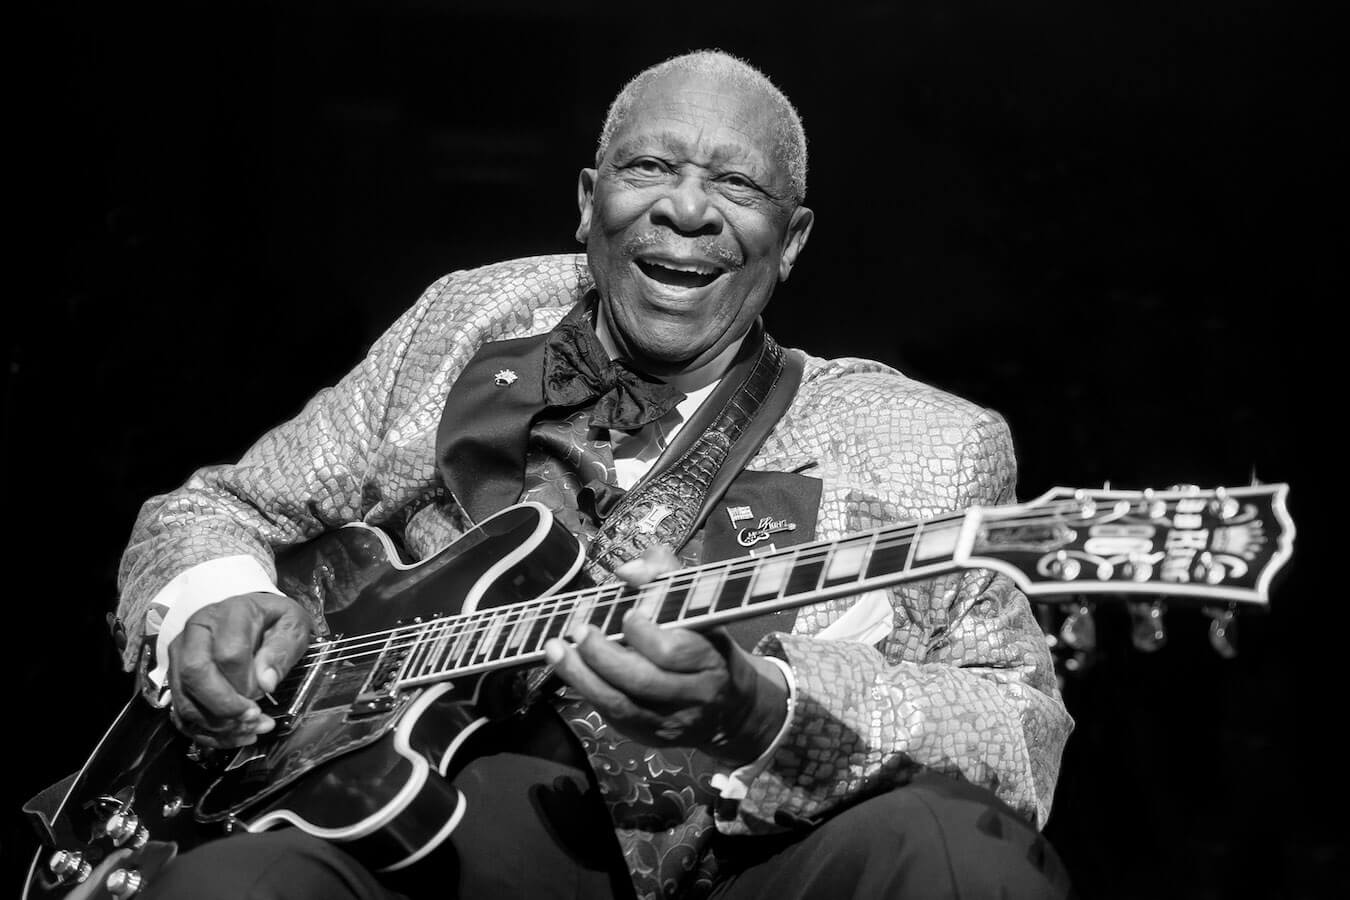
\includegraphics[width=1in,height=1.25in,clip,keepaspectratio]{author/bb-king.jpg}}]{B.B. King}\\
        is a world famous blues musician. 
\end{IEEEbiography}

\begin{IEEEbiography}[{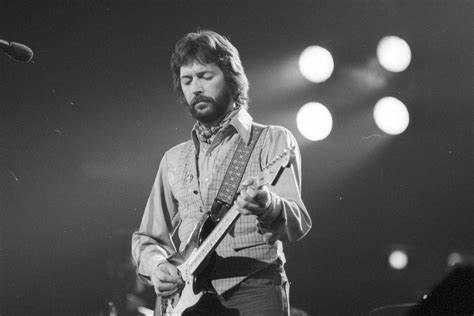
\includegraphics[width=1in,height=1.25in,clip,keepaspectratio]{author/EC.jpg}}]{Eric Clapton}\\
        is a famous musician. 
\end{IEEEbiography}
\end{document}